\section{Soziale Kontakte}
Nur gemeinsam sind wir stark! Im Studium kommen viele Herausforderungen auf euch zu, die gemeinsam leichter zu bewältigen sind und zudem sogar Spaß machen können. Es ist daher umso wichtiger, gleich zu Anfang Kontakte zu knüpfen. Das könnt ihr \zB beim Rahmenprogramm des Vorkurses (siehe \autopageref{vorkurs-rahmenprogramm}). Oder auch in den Tutorien, die in Kleingruppen stattfinden werden.

Beim berühmt-berüchtigten Zettelrechnen könnt ihr euch mit anderen Studierenden austauschen und euch gegenseitig helfen. Jede Woche werdet ihr pro Veranstaltung ein Übungsblatt bearbeiten und abgeben. Alleine verzweifelt man schnell und braucht sehr viel Zeit, gemeinsam kommt man schneller ans Ziel. Und wenn es manchmal sehr knifflig ist, haben mehre Köpfe meistens auch mehr gute Ideen. Und man profitiert ungemein davon, auch mal andere Lösungswege und Herangehensweisen an ein Problem zu sehen. Sich gegenseitig zu unterstützen und gemeinsam zu lernen gehört zum Studium einfach dazu.

Habt ihr einmal nette Menschen getroffen, können wir euch nur empfehlen, mit den anderen etwas zusammen zu unternehmen -- trotz des teilweise sehr stressigen Uni-Alltags. Trefft euch doch einfach mal zum Kochen, zum Wandern, Klettern, Volleyball spielen, zu Spieleabenden, zum Telefonieren oder was euch sonst noch so einfällt. Denn alleine fühlen solltet ihr im Studium nicht und müsst es auch nicht.

\begin{figure}[hb]
    \centering
    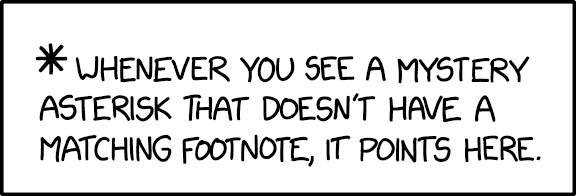
\includegraphics[width=0.8\linewidth]{bilder/mystery_asterisk_destination_2x.png}
\end{figure}

\vfill
